\chapter{Plano de manutenção}
\label{plano_de_manutenção}
\section{Os objetivos}
A manutenção de um sistema/software é fundamental no seu ciclo de vida e representa uma grande quantidade do seu tempo e esforço.\\
Tem como objetivo modificar o nosso produto depois de ser lançado ao público, para melhorar o seu desempenho, para corrigir falhas ou para adaptar ás mudanças no ambiente.\\
Nós queremos que o nosso software tenha uma vida contínua e longa depois do seu lançamento, mas ao mesmo tempo não queremos encontrar muitos obstáculos pelo caminho, especialmente aqueles postos em nós mesmos e para isso temos que evitar certos erros nesta fase de desenvolvimento como a sua documentação e planeamento.
\section{O nosso plano}
O nosso plano de manutenção é baseado num modelo estruturado que visa a passar por várias fases organizadas de maneira a que haja uma total eficiência na manutenção do nosso sistema e faz parte das 4 categorias que vamos usar.

\begin{figure}[H]
	\centering
	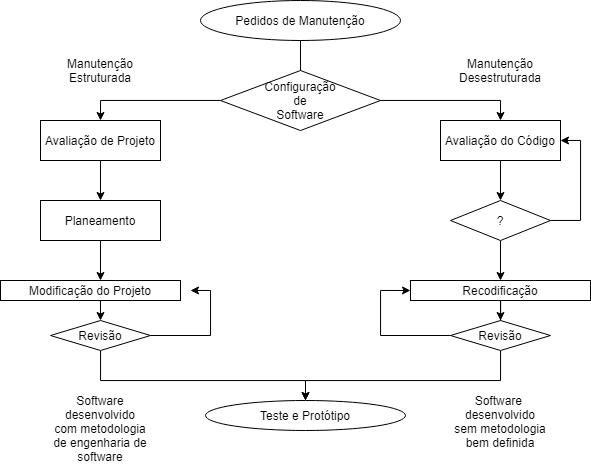
\includegraphics[width=15cm]{Pedidos_Manutencao}
	\caption{Manutenção estruturada e não estruturada}
	\label{fig:Pedidos_Manutencao}
\end{figure}

\subsection{As categorias de manutenção}
-Manutenção corretiva:\\
Tem como objetivo encontrar, identificar e corrigir os erros.\\
\\-Manutenção adaptativa:\\
É a adaptação do software ao ambiente.\\
\\-Manutenção perfectiva:\\
Baseia-se no atendimento a pedidos de utilizadores e "feedback" para modificar funcionalidades ou adicionar novas com fim de melhorar o sistema.\\
\\-Manutenção preventiva:\\
Esta ocorre normalmente durante o desenvolvimento do sistema, é preparar e melhorar a manutenibilidade, fornecendo uma boa fundação para conseguir fazer adaptações e futuros melhoramentos.

\subsection{Ações e equipas}
Para conseguirmos uma manutenção efetiva pós lançamento temos que primeiro estabelecer uma equipa focada nessa secção. Dado que de momento só existe a nossa equipa de 3 membros, também seremos a equipa de manutenção até quando houver a opção de aumentar a nossa equipa e ou designar uma equipa só mesmo focada na manutenção.\\
De seguida teriam que ser descritos procedimentos de avaliação, comunicação.\\
Depois é feita a descrição e definição de eventos sequenciais.\\

\begin{figure}[H]
	\centering
	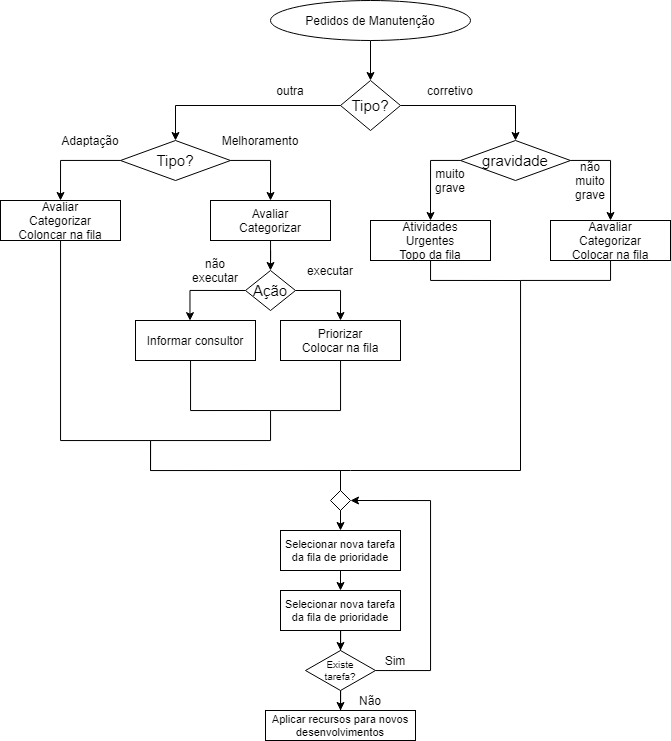
\includegraphics[width=15cm]{Pedidos_Manutencao_2}
	\caption{Sequência de eventos}
	\label{fig:Pedidos_Manutencao_2}
\end{figure}
\\
Em continuação, estabelecemos procedimentos para registrar o histórico de atividades feitas na manutenção e depois definimos critérios de avaliação e revisão.